\begin{figure}[!htbp]
    \begin{subfigure}{.5\textwidth}
        \centering
        \label{fig:pubmed_submission_per_year}
        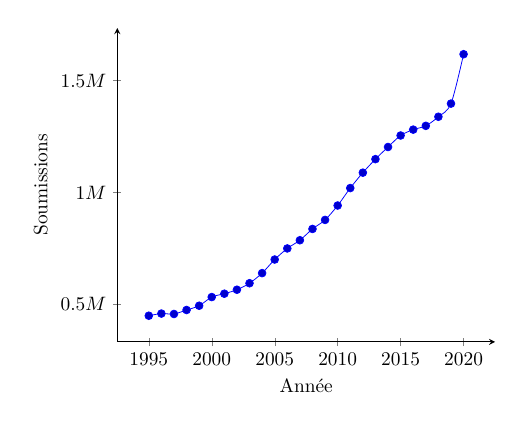
\begin{tikzpicture}[scale=0.7, transform shape]
        \begin{axis}[
        scaled y ticks=manual:{}{\pgfmathparse{#1/1000000}},
        axis x line=bottom, axis y line=left,
        enlargelimits=true,
        yticklabel=${\pgfmathprintnumber{\tick}M}$,
        xlabel=\text{Année},ylabel=\text{Soumissions},
        x tick label style={
            /pgf/number format/.cd, use comma, 1000 sep={},
        }]
        \addplot+[smooth] coordinates {
            (1995, 449050)(1996, 458678)(1997, 456812)(1998, 474666)(1999, 493712)(2000, 532503)(2001, 547504)(2002, 565256)(2003, 594340)(2004, 639530)(2005, 700229)(2006, 749769)(2007, 786530)(2008, 836935)(2009, 877310)(2010, 941684)(2011, 1019685)(2012, 1088548)(2013, 1148929)(2014, 1203202)(2015, 1254639)(2016, 1280910)(2017, 1297742)(2018, 1338381)(2019, 1397240)(2020, 1617944)
            };    
        \end{axis}
        \end{tikzpicture}
        \caption{PubMed}
    \end{subfigure}%
    %
    \begin{subfigure}{.5\textwidth}
        \centering
        \label{fig:arxiv_submission_per_year}
        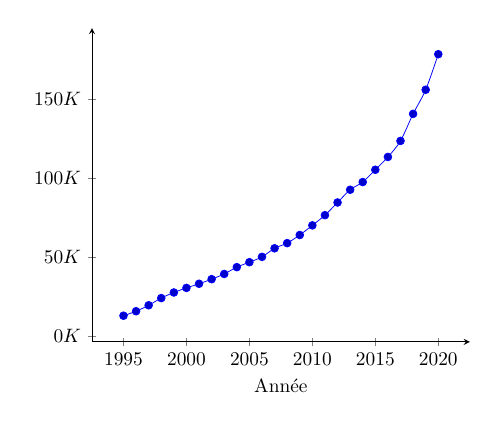
\begin{tikzpicture}[scale=0.7, transform shape]
        \begin{axis}[
            scaled y ticks=manual:{}{\pgfmathparse{#1/1000}},
            axis x line=bottom, axis y line=left,
            enlargelimits=true,
            yticklabel=${\pgfmathprintnumber{\tick}K}$,
            xlabel={Année},%ylabel=\text{Soumissions},
            x tick label style={
                /pgf/number format/.cd, use comma, 1000 sep={},
            }]
        \addplot+[smooth] coordinates {
            %(1991, 306)(1992, 3263)(1993, 6743)(1994, 10097)
            (1995, 13014)(1996, 15866)(1997, 19624)(1998, 24172)(1999, 27704)(2000, 30601)(2001, 33214)(2002, 36121)(2003, 39414)(2004, 43727)(2005, 46855)(2006, 50227)(2007, 55638)(2008, 58915)(2009, 64047)(2010, 70131)(2011, 76578)(2012, 84603)(2013, 92641)(2014, 97517)(2015, 105280)(2016, 113380)(2017, 123523)(2018, 140616)(2019, 155866)(2020, 178329)
            };    
        \end{axis}
        \end{tikzpicture}
        \centering
        \caption{ArXiv}
    \end{subfigure}%
    
    \iffalse
    \begin{subfigure}{.5\textwidth}
        \centering
        \label{fig:hal_submission_per_year}
        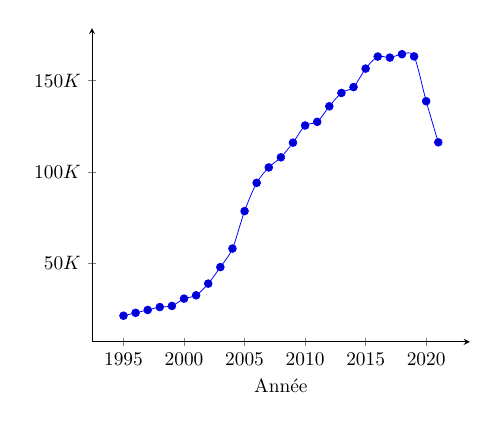
\begin{tikzpicture}[scale=0.7, transform shape]
        \begin{axis}[
            scaled y ticks=manual:{}{\pgfmathparse{#1/1000}}, 
            axis x line=bottom, axis y line=left,
            enlargelimits=true,
            yticklabel=${\pgfmathprintnumber{\tick}K}$,
            xlabel={Année},%ylabel=\text{Soumissions},
            x tick label style={
                /pgf/number format/.cd, use comma, 1000 sep={},
            }]
        \addplot+[smooth] coordinates {
            (2021, 116139)(2020, 138691)(2019, 163279)(2018, 164475)(2017, 162607)(2016, 163185)(2015, 156587)(2014, 146438)(2013, 143213)(2012, 135893)(2011, 127362)(2010, 125351)(2009, 115950)(2008, 107903)(2007, 102352)(2006, 93887)(2005, 78390)(2004, 57840)(2003, 47662)(2002, 38605)(2001, 32185)(2000, 30366)(1999, 26367)(1998, 25741)(1997, 24139)(1996, 22571)(1995, 20987)
            };    
        \end{axis}
        \end{tikzpicture}
        \centering
        \caption{HAL}
    \end{subfigure}
    \fi
    
    \caption{Nombre de nouveaux documents par an dans deux bibliothèques numériques scientifiques.}
    \label{fig:submission_per_year}
\end{figure}